\documentclass{article}
\usepackage{fancyhdr}
\usepackage{amsmath}
\usepackage{amsthm}
\usepackage{amssymb}
\usepackage{graphicx}
\usepackage{float}
\usepackage{subcaption}
\usepackage{hyperref}
\usepackage{listings}
\usepackage{color}
\usepackage{tikz}
\usepackage{pgfplots}
\usepackage{pgfplotstable}
\usepackage{listings}
\usepackage{color}
\usepackage{tikz}
\usepackage{amsthm}
\usepackage[margin=15mm]{geometry}

\definecolor{dkgreen}{rgb}{0,0.6,0}
\definecolor{gray}{rgb}{0.5,0.5,0.5}
\definecolor{mauve}{rgb}{0.58,0,0.82}

% Set up fancy header
\pagestyle{fancy}
\fancyhf{} % Clear default header and footer
\rhead{Keith Wesa} % Right header
\lhead{MAT Written Assingment 2:} % Left header
\rfoot{Page \thepage} % Right footer

\author{Keith Wesa}
\title{MAT 215 - Written Homework 1}
\date{\today}

\begin{document}

\section*{Question 1}

\subsection*{\textbf{Answer each of the following \newline [12 marks]}}
\begin{itemize}
    \item[a.] Consider the numbers 8, 13, 35, 46. Compute the sum and difference of each
    possible pairing (e.g. 8 and 13, 8 and 35, etc.). [Note: You don’t need to
    double up, e.g. you don’t need to do 8 + 13 and 13 + 8 because we know
    they are the same] What do you notice about the results (regarding even and
    odd)?
\end{itemize}

\begin{table}[!htb]
    \caption{Sum and difference for Question 1.a.}
    \begin{minipage}{1.0\linewidth}
      \label{tab:table_label}
      \begin{center}
        \begin{tabular}{ l | l | l | l }
            \textbf{Addition} & \textbf{Subtraction} & {Even} & {Odd} \\ \hline
            8+13 = 21  & 8-13 = -5 & -38 & -33 \\
            8+35 = 43 & 8-35 = -27 & -22 & -27 \\
            8+46 = 54 & 8-46 = -38 & 22 & -11 \\
            13+35 = 48 & 13-35 = -22 & 38 & -5 \\
            13+46 = 59 & 13-46 = -33 & 48 & 5 \\
            35+46 = 81 & 35-46 = -11 & 54 & 11 \\
                       & 13 - 8 = 5  & & 21 \\
                       & 35 - 8 = 27 & & 27 \\
                       & 46 - 8 = 38 & & 33 \\
                       & 35 - 13 = 22 & & 43 \\
                       & 46 - 13 = 33 & & 59\\
                       & 46 - 35 = 11 & & 81\\       
        \end{tabular}
    \end{center}
    \end{minipage}%
\end{table}
     
\begin{itemize}
    \item[] \textbf{Answer:} What I noticed by the results was, that whenever I had an 
    even number added to an odd number I got an odd number back. What I also noticed was 
    whenever I added an even by an even and even or odd and an odd I got an even back. 
\end{itemize}
Let n, m be even numbers, and p, q be odd numbers. (Hint: It will be useful for
parts b - d. to use a general representation of even and odd numbers.)
\begin{itemize}
    \item[b.] Prove that $n + m$ and $n - m$ are even.
    \item[] 
    \begin{proof}
        Let $n$ and $m$ be even and $\mathbb{Z}$. We will also call $k$ and $l$ any $\mathbb{Z}$. 
        Since, $n$ and $m$ are even we can say that $n = 2k$ and $m = 2l$.
        \begin{align*}
            n \pm m &= 2k \pm 2l \\
            &= 2(k \pm l) \\
            z &= k \pm l \\
            n \pm m &= 2z \\
        \end{align*}
        Since an even number is defined by any integer multiplied by two.\newline
        \textbf{Therefore:} $n + m$ and $n - m$ are even.
       
    \end{proof}
    \item[]
    \item[c.] Prove that $p + q$ and $p - q$ are odd.
    \item[]
        \begin{proof}
            Let $p$ and $q$ be odd and $\mathbb{Z}$. We will also call $k$ and $l$ any $\mathbb{Z}$. 
            Since, $p$ and $q$ are odd we can say that $p = 2k + 1$ and $q = 2l + 1$.
            \begin{align*}
                p \pm q &= 2k + 1 \pm 2l + 1 \\
                &= 2k \pm 2l + 2 \\
                &= 2(k \pm l + 1) \\
                z &= k \pm l + 1 \\
                p \pm q &= 2z \\
            \end{align*}
            Since an odd number is defined by any integer multiplied by two plus one, when we put those values together we
            can factor out a two assign a new variable to the function $ z = k \pm l + 1$ because it will just become an integer
            and two times any integer is even.
            \item[]
            \textbf{Therefore:} $p + q$ and $p - q$ are even.
        \end{proof}
    \item[d.] Prove that $n + p$ and $n - p$ are odd.
    \item[]
    \begin{proof}
        Let $n$ be even and $p$ be odd and $\mathbb{Z}$. We will also call $k$ and $l$ any $\mathbb{Z}$.
        Since, $n$ and $p$ are even and odd we can say that $n = 2k$ and $p = 2l + 1$.
        \begin{align*}
        n \pm p &= 2k \pm 2l + 1 \\
        &= 2(k \pm l) + 1 \\
       z &= k \pm l \\
       n \pm p &= 2z + 1 \\
        \end{align*}
    Since we are adding or subtracting the integer $n$ and $p$ together will result in $2(k \pm l) + 1$ and
    we set $z = (k \pm l)$ our result will be $2z \pm 1 \equiv 2k \pm 1$ 
    \item[]
        \textbf{Therefore} $n + p$ are $n - p$ are odd
    \end{proof}
\end{itemize}
for each statement below, find a counterexample.
\begin{itemize}
    \item[e.] If the sum of one pair of positive integers is larger than the sum of another
    pair, then the product is also larger.
    \item[] 
        \textbf{answer:} If the sum of one pair of positive integers is larger then the sum of another 
        pair, then the product is equal.
    \item[f.] If the product of one pair of positive integers is larger than the product of
    another pair, then the sum is also larger.
    \item[]
        \textbf{answer:} If the product of on pair of positive integers is larger than the product of 
        another pair, then the sum is smaller.
\end{itemize}
\section*{Question 2}
\subsection*{\textbf{Answer each of the following} \newline {[10 marks]}}

\begin{itemize}
    \item[a.] Prove that we cannot write $n^4 - n$ as a product of four consecutive numbers
    (thus showing that the two generalizations are no longer equivalent)? (Hint:
    Factor $n^4 - n$.)
    \begin{proof}
        \begin{align*}
            n^4 - n &= n(n^3 - 1) \\
            &= n(n^3 - 1^3) \\
            &= n(n - 1)(n^2 + n + 1)\\
            &= (n - 1)(n)(n + 1)(n + 2) \\
            n(n - 1)(n^2 + n + 1) &\neq (n - 1)(n)(n + 1)(n + 2) \\ 
            0 &= n(n - 1) \\
            n &= 1 \\
            n &= 0 \\
            0 &= n^2 + n + 1 \\
            n &= \frac{-1 \pm \sqrt{1 - 4(1)(1)}}{2(1)} \\
            n &= \frac{-1 \pm \sqrt{-3}}{2} \\
            n &= \frac{-1 \pm i\sqrt{3}}{2}, 0, 1 \\                  
        \end{align*}
        \item[] \textbf{Contradiction:} What I'm attempting to show is that $n^4 - n$ can't be a product of four consecutive numbers.
        by showing 
        \begin{itemize}
            \item[1.] $n(n - 1)(n^2 + n + 1) \neq (n - 1)(n)(n + 1)(n + 2)$
            \item[2.] That the roots of $n^4 - n$ are not consecutive numbers. If the roots had been consecutive numbers the statement would have been true.
        \end{itemize}
        \item[] \textbf{Therefore:} We cannot write $n^4 - n$ as a product of four consecutive numbers        
    \end{proof}
    \item[]   
    \item[b.]  Is $n^4 - n$ divisible by 4? Show your work.
    \begin{proof}
        \begin{align*}
            &= \frac{n^4 - n}{4} \\
            &= \frac{n(n - 1)(n^2 + n + 1)}{4} \\
            f(x) &= \frac{n}{4} \\
            g(x) &= \frac{n - 1}{4} \\
            h(x) &= \frac{n^2 + n + 1}{4} \\
        \end{align*}
    \end{proof}
    \item[] \textbf{Answer:} $n^4 - n$ is divisible by 4. For all even numbers $n$, or $n = 4k + 1$.
    \item[]
    \item[c.] Is the product of four consecutive numbers divisible by 4? Is the product of 5 
    consecutive numbers divisible by 5?
    \item[]
    \item[] \textbf{Answer:} Yes the product of 4 consecutive numbers is divisible by 4. Yes the product of 5 consecutive numbers is divisible by 5.
    \begin{proof}
        \begin{align*}
            \frac{4!}{4} &= 6 \\
            \frac{5!}{5} &= 24 \\
        \end{align*}
    \end{proof}
    \item[]
    \item[d.] Formulate a conjecture about the product of n consecutive numbers.
    \item[] \textbf{Answer:} The product of $n$ consecutive numbers is divisible by $n$ for all $n \in \mathbb{Z}$
    \begin{proof}
        \begin{align*}
            \frac{n!}{n} &= \frac{n(n - 1)(n - 2)(n - 3)...(n - n)}{n} \\
            \frac{n!}{n} &= (n - 1)(n - 2)(n - 3)...(n - n) \\
        \end{align*}
    \end{proof}
    \item[] 
    \item[e.] Formulate four additional generalizations to our second main elementary fact.
    \item[] \textbf{Answer:}
    \item[] The product of $n$ consecutive numbers is divisible by $n$ for all n as long as n is an integer $\forall n \exists k \in \mathbb{Z}(\frac{n!}{n}=k)$ 
     
\end{itemize}
\section*{Question 3}

\subsection*{\textbf{Answer each of the following \newline [8 marks]}}
\begin{itemize}
    \item[]
    \item[a.] Critique the following argument.
    \item[] 
    \item[] \textbf{Statement:} for any natural number, $n^3 - n$ is even. \textit{look for logical mistakes}
    \item[] 
    \item[] \textbf{Answer:} The statement reads poorly, When using Quantifiers you should define the variable, also the statement "For any" is not really quantifier.
    \item[] \textbf{Corrected Statement:} For all values of n, n being a natural number, $n^3 - n$ is even. \textit{Alternatively} $\forall n \in \mathbb{N} (n^3 - n = 2k)$.

\end{itemize}
\textbf{Theorem (1)} for any natural number, $n^3 - n^2$ is even.
\begin{itemize}
    \item[b.] Prove the theorem using algebra.
    \item[] 
    \begin{proof}
        Let $n$ be a natural number and $\mathbb{Z}$. We will also call $k$ any $\mathbb{Z}$. 
        Since, $n$ is a natural number we can say that $n = 2k$.
        \begin{align*}
            n^3 - n^2 &= (2k)^3 - (2k)^2 \\
            &= 8k^3 - 4k^2 \\
            &= 4k^2(2k - 1) \\
            &= 2(2k^2)(2k - 1) \\
            z&= 2k^2(2k - 1) \\
            &= 2z \\
            n^3 - n^2 &= 2z \\
        \end{align*}
        Since an even number is defined by any integer multiplied by two.\newline
        \textbf{Therefore:} $n^3 - n^2$ is even.
    \end{proof}
    % \newpagef
    \item[c.] Prove the theorem using geometry.
    \item[]
    \begin{proof}

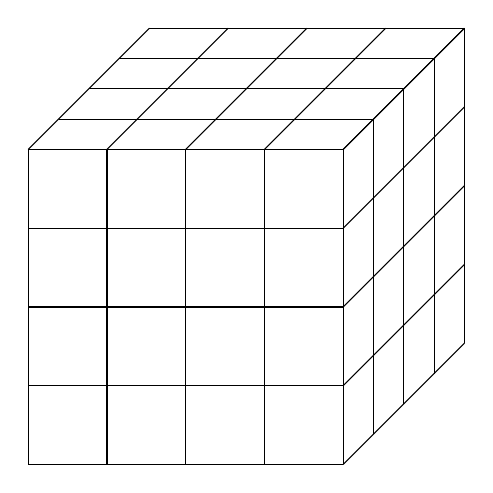
\begin{tikzpicture}
\foreach \x in{0,...,4}
{   \draw (0,\x ,4) -- (4,\x ,4);
    \draw (\x ,0,4) -- (\x ,4,4);
    \draw (4,\x ,4) -- (4,\x ,0);
    \draw (\x ,4,4) -- (\x ,4,0);
    \draw (4,0,\x ) -- (4,4,\x );
    \draw (0,4,\x ) -- (4,4,\x );
}
\end{tikzpicture}

\begin{tikzpicture}
    \draw[step=1cm,gray!50!white,very thin] (0,0) grid (4,4);
    \draw[thick] (0,0) -- (4,0) -- (4,4) -- (0,4) -- cycle;
    \draw[thick] (0,0) -- (0,4);
    \draw[thick] (4,0) -- (4,4);
\end{tikzpicture}
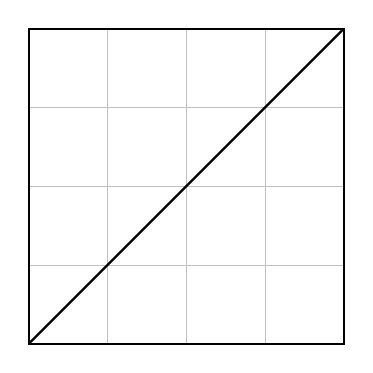
\begin{tikzpicture}
    \draw[step=1cm,gray!50!white,very thin] (0,0) grid (4,4);
    \draw[thick] (0,0) -- (4,0) -- (4,4) -- (0,4) -- cycle;
    \draw[thick] (0,0) -- (0,4);
    \draw[thick] (4,0) -- (4,4);
    \draw[thick] (0,0) -- (4,4);
\end{tikzpicture}
\item[]
\item[] \textbf{Answer:} Alright here is where I give up on trying to make a text editor display the imagine in my brain. 
So I'll just explain it from here. We have a 4x4 grid of squares which we can consider a plane. I we were to take that plane and
bisect the cube diagonally we would get two 3D triangles which is even because the grid is is symmetrical. It would look like the 
third image if you were staring directly at it.
\end{proof}
\end{itemize}    
\end{document}